\documentclass[onecolumn,12pt]{IEEEtran}
\usepackage[utf8]{inputenc}
\usepackage[left=1in,right=1in,bottom=0.95in,nohead,nofoot]{geometry}
\usepackage{graphicx}

\begin{document}
\title{Informe Laboratorio 6}
\author{Redes de Datos}
%\vspace{3mm}

\begin{figure}[h]

\includegraphics[width=0.50\textwidth]{logo_udp.png}
\label{fig:mesh1}
\\
\\
\\
\\
\\
\maketitle
\end{figure}
\begin{center}
Integrantes:\\
\hfill \\
Gonzalo Calderón\\
Andrés Hernández\\
Franco Centeno\\
\hfill \\
\hfill \\
\hfill \\
\hfill \\
\ \hfill \\
Profesor:\\
Jose Perez\\ \hfill \\
Ayudante:\\
Alexis Inzunza\\
\hfill \\
\hfill \\
\hfill \\
\hfill \\
\hfill \\
26 de Mayo de 2017
\end{center}

\newpage
\title{Indice}
\author{ }
\maketitle
\hrule
\tableofcontents

\newpage
\section{INTRODUCCIÓN}
\hfill \\

En este laboratorio trabajamos con sockets, lo cuales son un mecanismo que permite el intercambio de información entre un cliente y un servidor. Para su utilización se necesitan dos identificadores, para los equipos a conectar (IP), un protocolo de transporte, el cual puede ser TCP o UDP, dependiendo de la necesidad. Mientras que TCP esta orientado más a la conexión, tiene confiabilidad en la entrega de mensajes, detección y corrección de errores, control de flujo y control de congestión, UDP no. Además se necesitan dos números de puerto (uno local y otro remoto).
 

\hfill \\
\section{ACTIVIDAD 1}
\hfill \\

La actividad consiste en crear un algoritmo utilizando Python. Se hizo uso de la librería "socket", basada en la API conocida como "Sockets de Berkeley", que es una implementación de los sockets.\\

El código del cliente usa las bibliotecas Socket y Threading, estás bibliotecas proporcionan comandos para conectarse a un servidor, y poder ejecutar multi-tareas. Gracias a la biblioteca Socket podemos utilizar las funciones "connect()", el cual sirve para conectarse al servidor, "send()" el cual sirve para enviar mensajes, "recv()" para recibir mensajes, entre muchos otros. Usamos el siguiente cliente en Python para poder probar nuestro servidor:

\begin{figure}[!h]
\centering
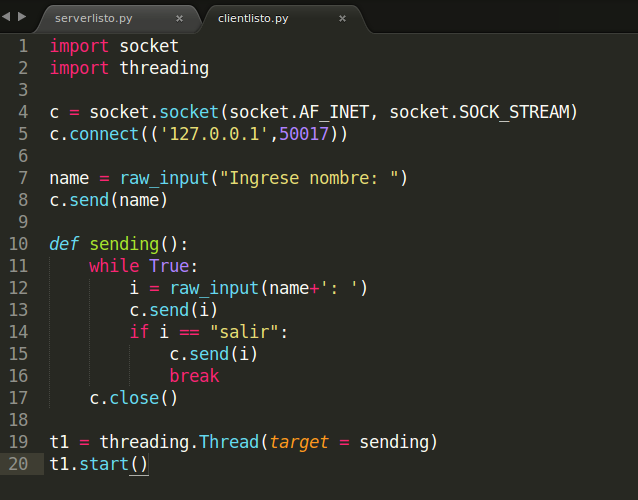
\includegraphics[width=0.6\textwidth]{clientesito.png}
\label{fig:mesh1}
\end{figure}
\\
\newpage
Luego creamos un servidor el cual tambien importa las bibliotecas Socket y Threading.

\begin{figure}[!h]
\centering
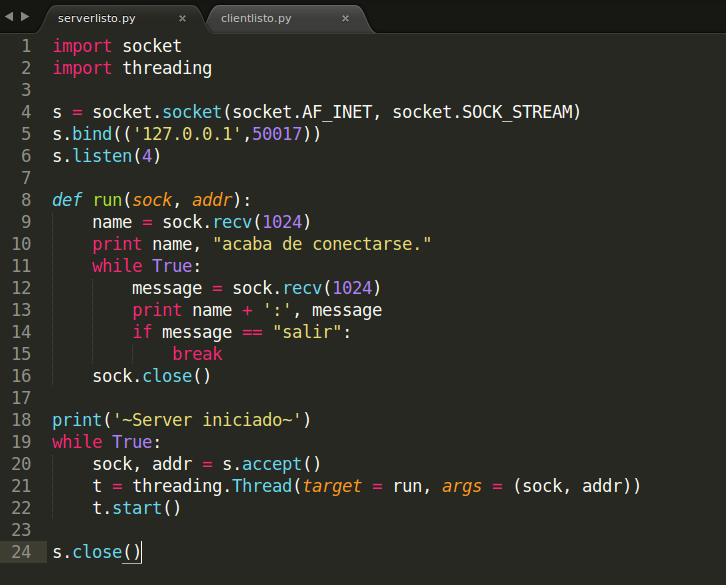
\includegraphics[width=0.6\textwidth]{servidorsito.png}
\label{fig:mesh1}
\end{figure}

\hfill \\
\section{ACTIVIDAD 2}
\hfill \\

Utilizando Wireshark, analizamos el tráfico de información al ejecutar el servidor y dos clientes, los clientes con distintas direcciones, y luego verificamos el funcionamiento del servidor, se enviaban mensajes correctamente desde ambos clientes, y el programa Wireshark podía leer los mensajes sin problemas, como se observa en la siguiente imagen:

\begin{figure}[!h]
\centering
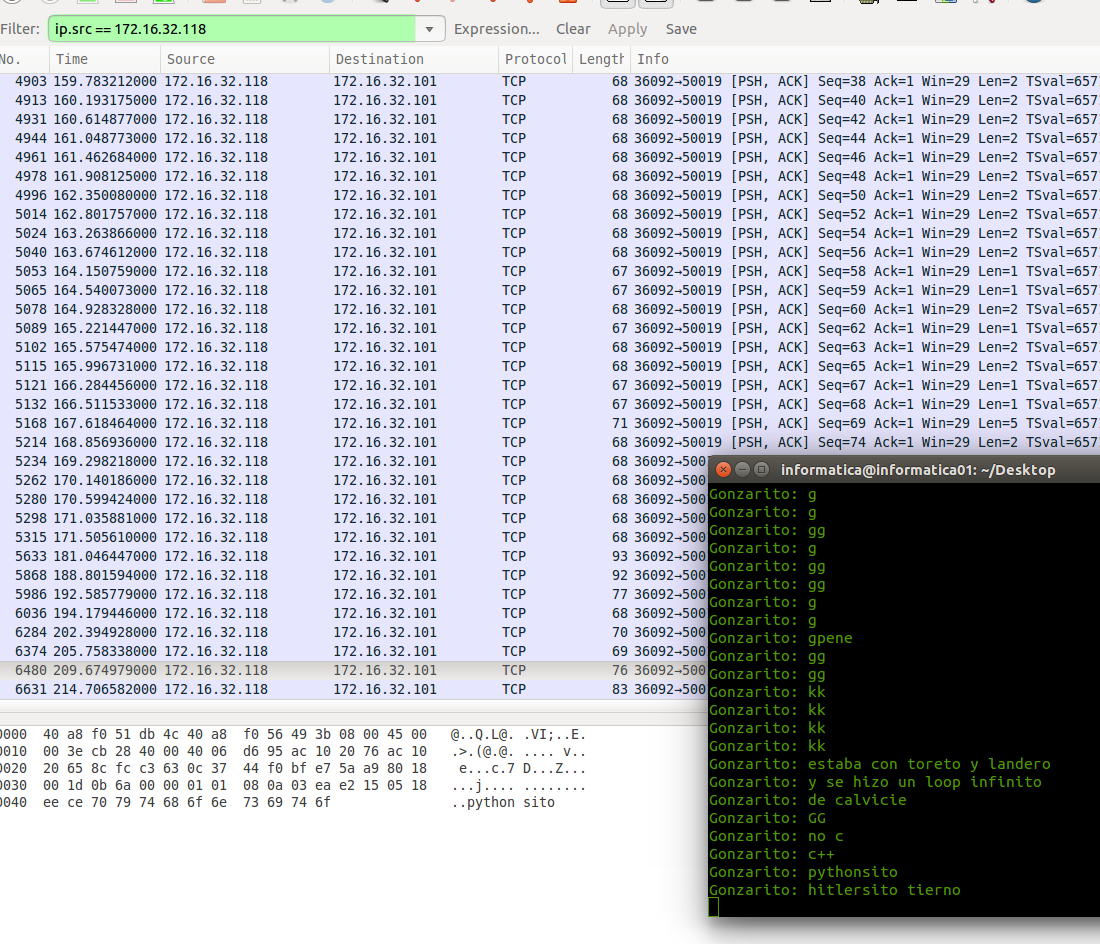
\includegraphics[width=0.6\textwidth]{wiresharkisito.png}
\label{fig:mesh1}
\end{figure}

\newpage
\hfill \\
\section{PREGUNTAS}
\hfill \\

1.- Utilizando la información obtenida en la actividad 2, explique el funcionamiento del envío y recepción de información para su algoritmo, respondiendo a las interrogantes ¿Qué se envía? ¿Cómo se envía?\\ \\
R: Se envian paquetes directamente desde el cliente al servidor, gracias a las funciones proporciadas por las bibliotecas anteriormente mencionadas.
\\ \\
2.- ¿Por qué el puerto que muestra el servidor al generar la conexión no es el mismo que el escrito en el
algoritmo del cliente?\\ \\
R: Porque al enviarse un mensaje e intentarlo verlo por el programa Wireshark, se crea un puerto aleatorio, por el cual se mostrará el mensaje.
\\ \\
3.- Si usted tuviese que realizar un videojuego con soporte multijugador utilizando sockets ¿Qué protocolo
utilizaría? ¿Por qué?\\ \\
R: TCP y UDP, ya que TCP se orienta mucho mas en la conexión, controla el flujo de mensajes y la congestión, es mucho más completo en lo que son los aspectos para varios hosts conectados a la vez y UDP cuando sea necesaria una transmisión de datos en tiempo real.
\\ \\
4.- ¿Se puede utilizar cualquier número de puerto para cualquier aplicación? Explique.\\ \\
R: No, ya que algunos están reservados para el sistema operativo y protocolos más utilizados y otros que son reservados a las aplicaciones que necesitan conectarse a un servidor y, por lo tanto, los que se utilizan en algunas de nuestras aplicaciones. Del 1024 al 49151 aproximadamente, son los puertos que se utilizan para la mayoría de aplicaciones y por norma general utilizaremos este rango a la hora de configurar nuestras conexiones.
\\ \\

\newpage
\section{CONCLUSIÓN}
\hfill \\

Con este laboratorio hemos podido comprender los sockets, protocolo TCP y UDP, su funcionamiento y caracteristicas. La forma en que transmiten los datos es una de sus principales diferencias, y serán las grandes determinantes para saber en qué se emplearán, dependiendo si se quiere una transmición segura, ordenada  y confiable, o en cambio, una transmisión de protocolos en los que el intercambio de paquetes de la conexión son mayores

\hfill \\
\hfill \\
\section{BIBLIOGRAFIA}
\hfill \\
TCP/UDP 
\emph{CCM} \\
\url{http://es.ccm.net/faq/1559-diferencias-entre-los-protocolos-tcp-y-udp}


\end{document} 
